\documentclass[11pt,ngerman]{article}

\renewcommand{\familydefault}{\sfdefault}

\usepackage[a4paper, top=1in, bottom=1in, left=1in, right=1in, headheight=15pt, asymmetric]{geometry}
\geometry{bindingoffset=2.1cm}

\usepackage{lipsum}
\usepackage{xcolor}
\usepackage{hyphenat}
\usepackage{graphicx}
\usepackage{sectsty}
\usepackage{amsmath}
\usepackage{amssymb}
\usepackage{stmaryrd}
\usepackage{fancyhdr}
\usepackage{ifxetex}
\usepackage{xifthen}

\ifxetex
    \usepackage{xltxtra}
    \usepackage{polyglossia}
    \usepackage{fontspec}
    \usepackage{titlesec}
    \usepackage[hidelinks,xetex]{hyperref}
    \usepackage[BoldFont,SlantFont]{xeCJK}
    \defaultfontfeatures{Mapping=tex-text}
    \setmainlanguage[spelling=new,babelshorthands=true]{german}
    \setCJKmainfont{IPAexMincho}
    \setCJKsansfont{IPAexGothic}
    \setCJKmonofont{IPAexGothic}
    \newcommand{\jap}[1]{#1}
\else
    \usepackage[utf8]{inputenc}
    \usepackage[T1]{fontenc}
    \usepackage[ngerman]{babel}
    \usepackage{CJKutf8}
    \newcommand{\jap}[1]{\begin{CJK}{UTF8}{min}#1\end{CJK}}
\fi

\titleformat{\section}{\normalfont\LARGE\centering}{\thesection}{1em}{}
\titleformat{\subsection}{\normalfont\Large\centering}{\thesubsection}{1em}{}
\titleformat{\subsubsection}{\normalfont\large\centering}{\thesubsubsection}{1em}{}
\titleformat{\paragraph}[runin]{\normalfont\large\centering}{\theparagraph}{1em}{}
\titleformat{\subparagraph}[runin]{\normalfont\large\centering}{\thesubparagraph}{1em}{}

\setlength{\parindent}{0in}
\sectionfont{\centering}

\newcommand{\commit}{\input{COMMIT}}
%\usepackage{xstring}
%\usepackage{catchfile}
%\CatchFileDef{\headfull}{.git/HEAD.}{}
%\StrGobbleRight{\headfull}{1}[\head]
%\StrBehind[2]{\head}{/}[\branch]
%\CatchFileDef{\commit}{.git/refs/heads/\branch.}{}

\fancypagestyle{style}{
    \fancyhf{}                          
    \fancyhead[LE]{\leftmark} %\slshape 
    \fancyhead[RO]{\rightmark} %\slshape
    \fancyfoot[LE]{\scriptsize\hyperlink{toc}{\thepage}}
    \fancyfoot[RO]{\scriptsize\hyperlink{toc}{\thepage}}
    \fancyfoot[RE]{\scriptsize\texttt{\commit}}
    \fancyfoot[LO]{\scriptsize\texttt{\commit}}
    %\fancyfoot[C]{\texttt{\scriptsize\commit}}
    \renewcommand{\headrulewidth}{0pt}  
    \renewcommand{\footrulewidth}{0pt}}
\pagestyle{style}

\definecolor{kanji}{HTML}{0d3481}
\definecolor{hiragana}{HTML}{8A1818}
\definecolor{katakana}{HTML}{086d3a}
\definecolor{romaji}{HTML}{000000}
\definecolor{german}{HTML}{000000}

\newcommand{\inputplaceholder}{{$\square$}}
\newcommand{\ifequals}[3]{\ifthenelse{\equal{#1}{#2}}{#3}{}}
\newcommand{\case}[2]{#1 #2}
\newenvironment{switch}[1]{\renewcommand{\case}{\ifequals{#1}}}{}

\input{tokens.tex}

\title{日本語}
\author{}
\date{}

\begin{document}

% -----------------------------------------------------------------------------

\begin{center}
    \Huge 日本語
\end{center}

\vfill

\begin{center}
    \textbf{Hiragana}
\end{center}

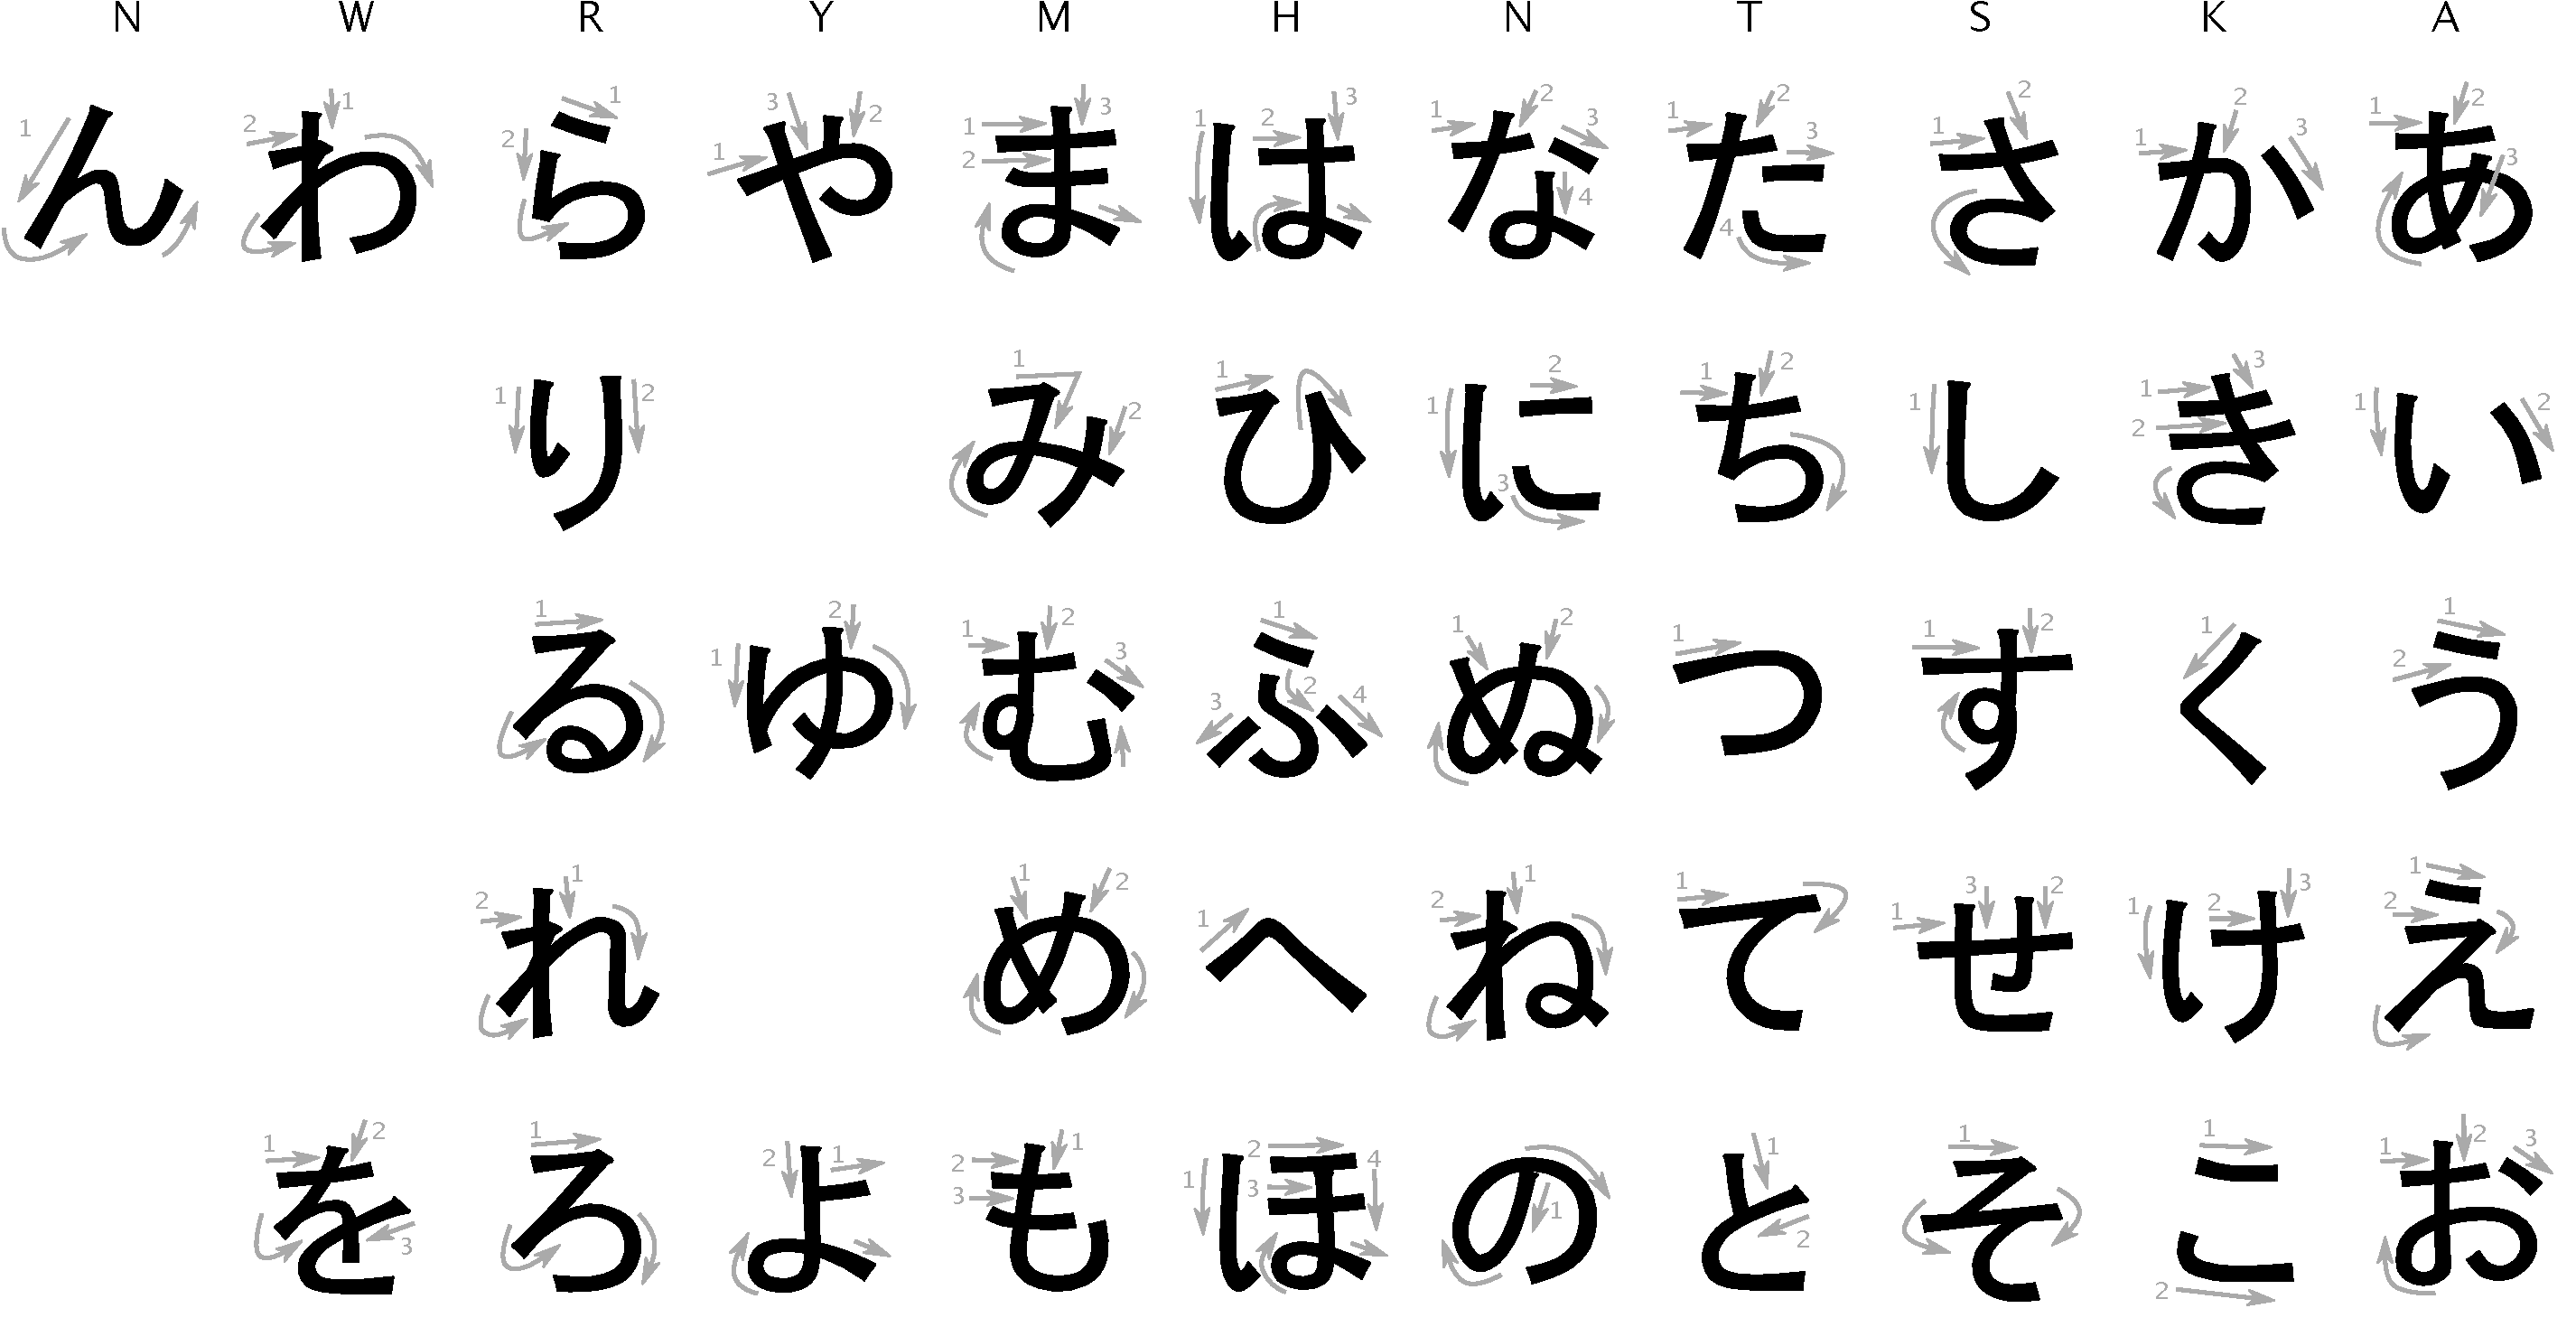
\includegraphics[width=\textwidth]{hiragana.pdf}

\bigskip
\bigskip

\begin{center}
    \textbf{Katakana}
\end{center}

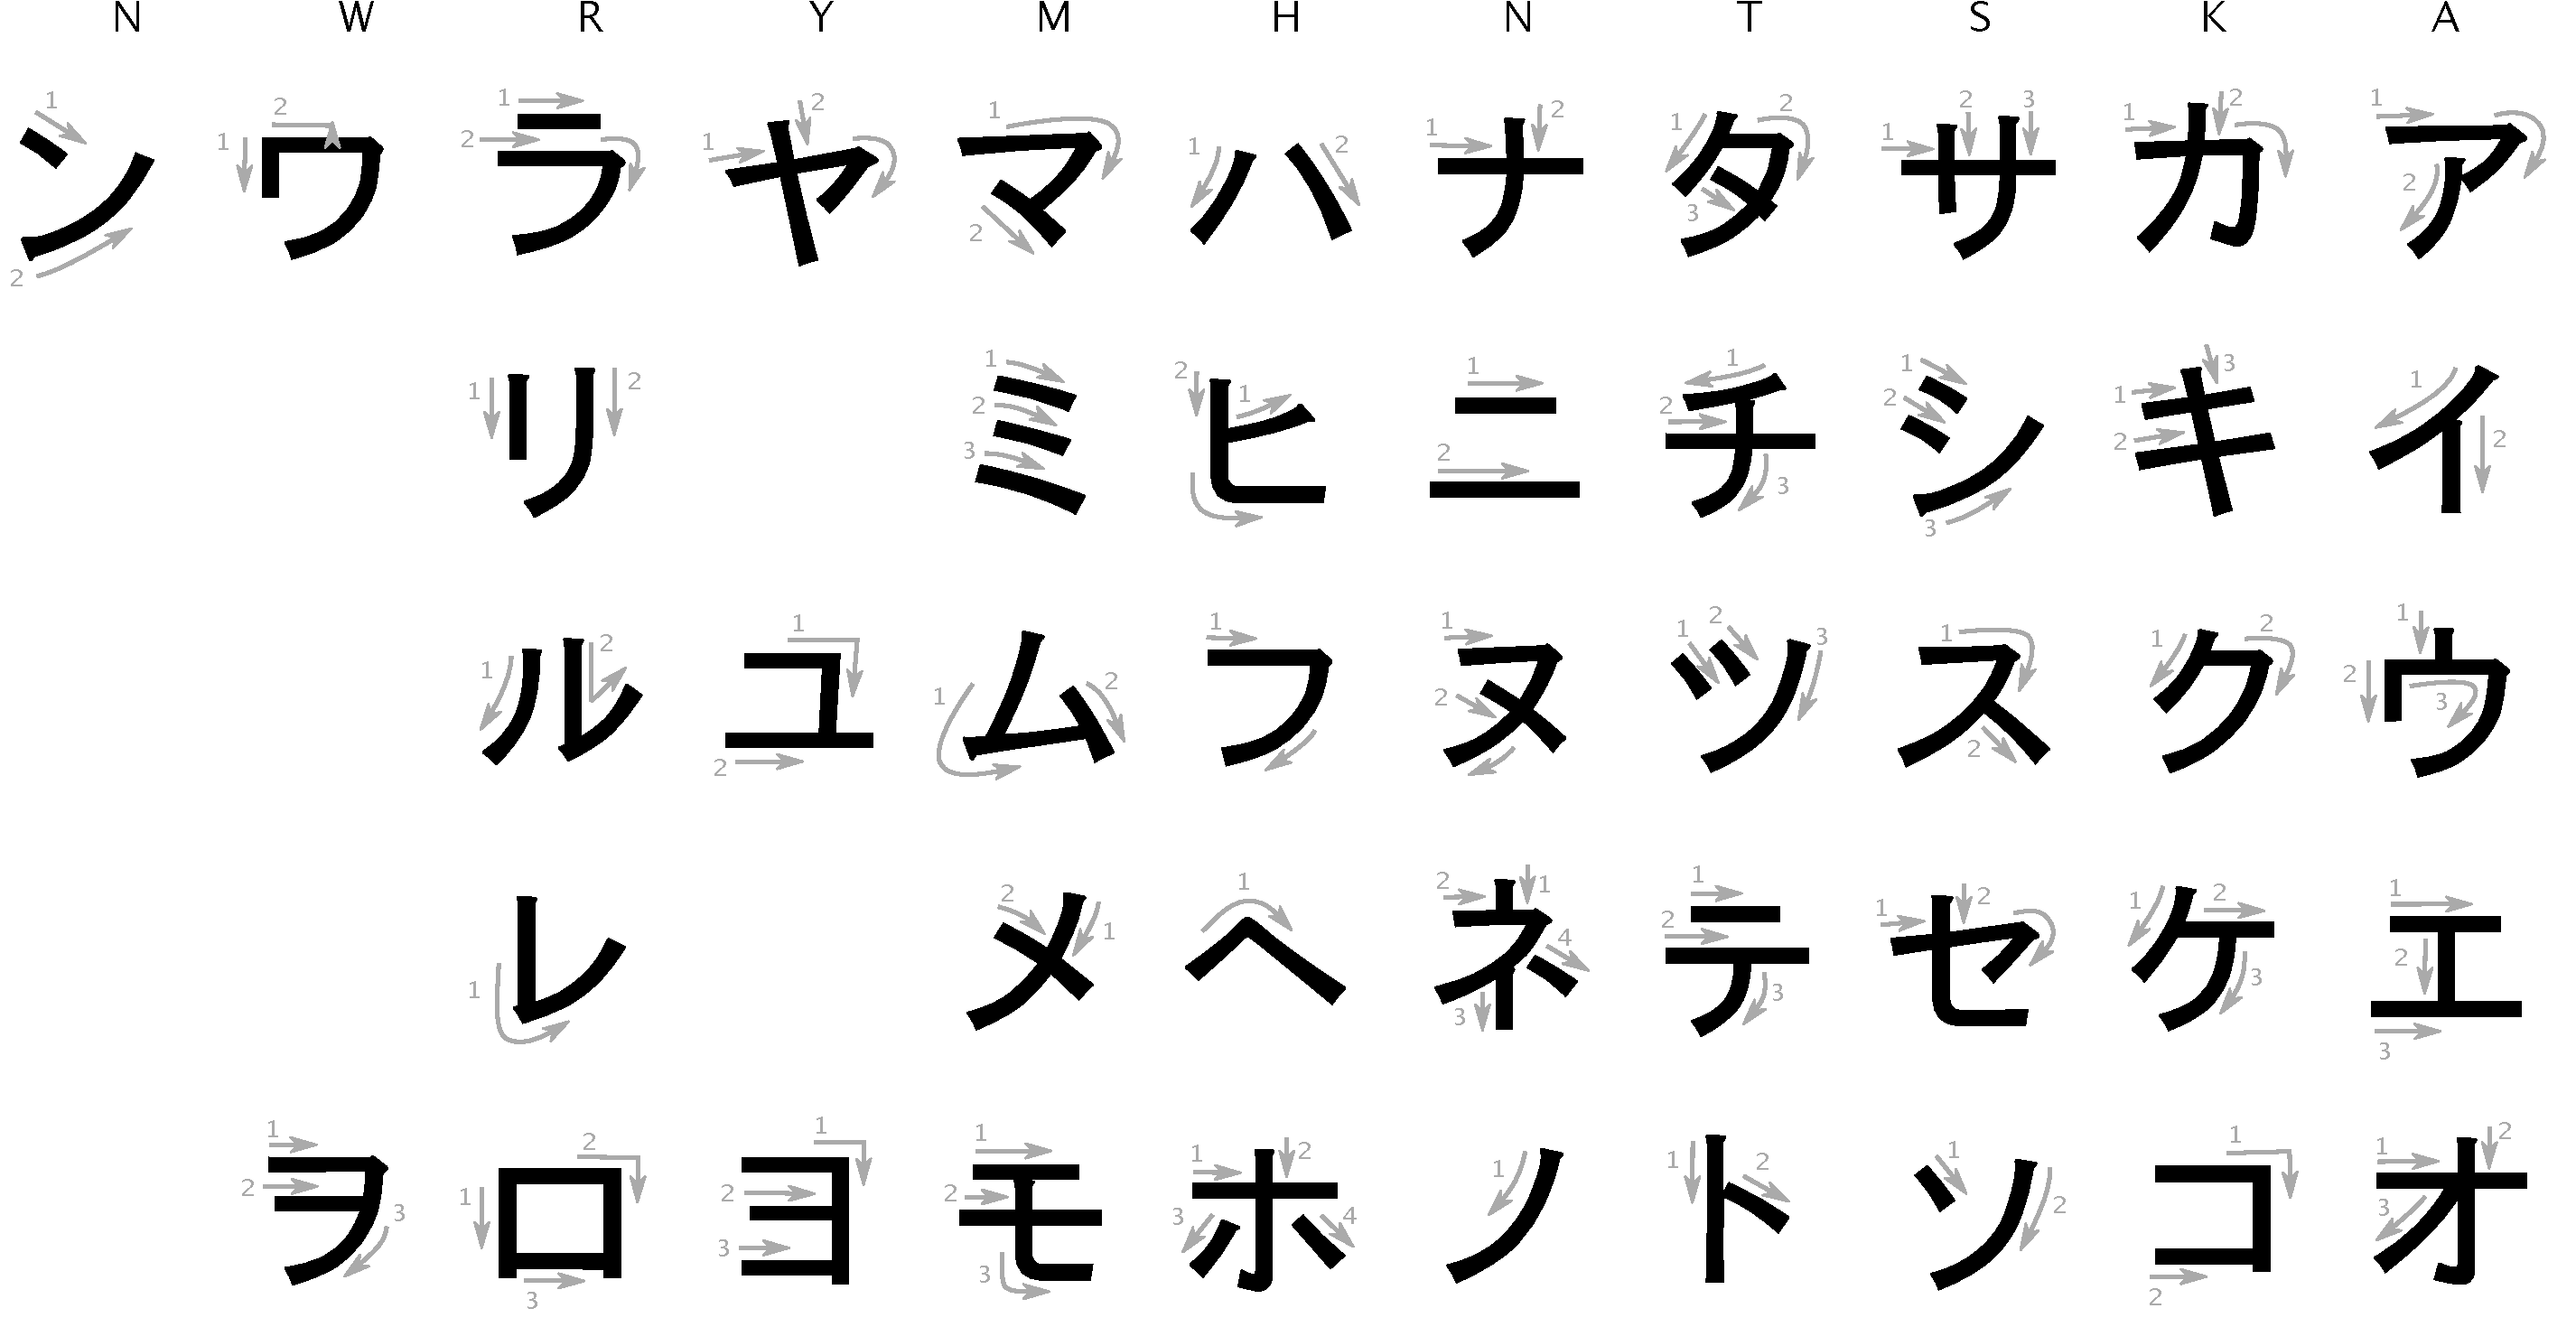
\includegraphics[width=\textwidth]{katakana.pdf}

\vfill

\newpage

% -----------------------------------------------------------------------------

\section*{日本語 A1.1 Zusammenfassung}

\subsection*{Gruß}

\begin{tabular}{@{}llll@{}}
\token{good_morning}{kanji}&\token{good_day}{kanji}&\token{good_evening}{kanji}&\token{goodbye}{kanji}\\
\token{good_morning}{hiragana}&\token{good_day}{hiragana}&\token{good_evening}{hiragana}&\token{goodbye}{hiragana}\\
\token{good_morning}{german}&\token{good_day}{german}&\token{good_evening}{german}&\token{goodbye}{german}\\
\end{tabular}

\bigskip

\token{nice_to_meet_you}{kanji}\\
\token{nice_to_meet_you}{hiragana}\\
\token{nice_to_meet_you}{german}

\bigskip

\subsection*{Unterricht}

\begin{tabular}{@{}ll@{}}
\token{lets_start_with_the_lessons}{kanji}&\token{we_are_done_for_today}{kanji}\\
\token{lets_start_with_the_lessons}{hiragana}&\token{we_are_done_for_today}{hiragana}\\
\token{lets_start_with_the_lessons}{german}&\token{we_are_done_for_today}{german}\\
\end{tabular}

\bigskip

\subsection*{Befinden}

\token{how_are_you}{kanji}\\
\token{how_are_you}{hiragana}\\
\token{how_are_you}{german}

\bigskip

\token{i_am_fine}{kanji}\\
\token{i_am_fine}{hiragana}\\
\token{i_am_fine}{german}

\bigskip

\begin{tabular}{@{}ll@{}}
\token{i_do_not_feel_good}{kanji}&\token{i_am_sick}{kanji}\\
\token{i_do_not_feel_good}{hiragana}&\token{i_am_sick}{hiragana}\\
\token{i_do_not_feel_good}{german}&\token{i_am_sick}{german}\\
\end{tabular}

\bigskip

\token{get_well}{kanji}\\
\token{get_well}{hiragana}\\
\token{get_well}{german}

\bigskip

\subsection*{Tee}

\begin{tabular}{@{}lll@{}}
\token{lets_trink_tea}{kanji}&\token{yes_of_course}{kanji}&\token{thank_you}{kanji}\\
\token{lets_trink_tea}{hiragana}&\token{yes_of_course}{hiragana}&\token{thank_you}{hiragana}\\
\token{lets_trink_tea}{german}&\token{yes_of_course}{german}&\token{thank_you}{german}\\
\end{tabular}

\bigskip

\begin{tabular}{@{}lll@{}}
\token{does_it_taste}{kanji}&\token{yes_it_tastes_good}{kanji}&\token{no_it_does_not_taste_good}{kanji}\\
\token{does_it_taste}{hiragana}&\token{yes_it_tastes_good}{hiragana}&\token{no_it_does_not_taste_good}{hiragana}\\
\token{does_it_taste}{german}&\token{yes_it_tastes_good}{german}&\token{no_it_does_not_taste_good}{german}\\
\end{tabular}

\bigskip

\subsection*{Selbstvorstellung}

\token{my_name_is}{kanji}\\
\token{my_name_is}{hiragana}\\
\token{my_name_is}{german}

\bigskip

\token{i_am_from}{kanji}\\
\token{i_am_from}{hiragana}\\
\token{i_am_from}{german}

\bigskip

\token{my_birthday_is}{kanji}\\
\token{my_birthday_is}{hiragana}\\
\token{my_birthday_is}{german}

\bigskip

\token{i_live_in}{kanji}\\
\token{i_live_in}{hiragana}\\
\token{i_live_in}{german}

\bigskip

%\token{i_am_gender}{kanji}\\
%\token{i_am_gender}{hiragana}\\
%\token{i_am_gender}{german}

\bigskip

\token{my_hobby_is}{kanji}\\
\token{my_hobby_is}{hiragana}\\
\token{my_hobby_is}{german}

\bigskip

\token{my_favorite_food_is}{kanji}\\
\token{my_favorite_food_is}{hiragana}\\
\token{my_favorite_food_is}{german}

\bigskip

\token{my_favorite_drink_is}{kanji}\\
\token{my_favorite_drink_is}{hiragana}\\
\token{my_favorite_drink_is}{german}

\bigskip

\token{my_favorite_ice_cream_is}{kanji}\\
\token{my_favorite_ice_cream_is}{hiragana}\\
\token{my_favorite_ice_cream_is}{german}

\bigskip

\token{my_favorite_fruit_is}{kanji}\\
\token{my_favorite_fruit_is}{hiragana}\\
\token{my_favorite_fruit_is}{german}

\bigskip

\token{my_favorite_color_is}{kanji}\\
\token{my_favorite_color_is}{hiragana}\\
\token{my_favorite_color_is}{german}

\bigskip

\subsection*{Datum}

\token{today_is}{kanji}\\
\token{today_is}{hiragana}\\
\token{today_is}{german}

\bigskip

\begin{tabular}{@{}lllllll@{}}
\token{monday}{kanji}&\token{tuesday}{kanji}&\token{wednesday}{kanji}&\token{thursday}{kanji}&\token{friday}{kanji}&\token{saturday}{kanji}&\token{sunday}{kanji}\\
\token{monday}{hiragana}&\token{tuesday}{hiragana}&\token{wednesday}{hiragana}&\token{thursday}{hiragana}&\token{friday}{hiragana}&\token{saturday}{hiragana}&\token{sunday}{hiragana}\\
\token{monday}{german}&\token{tuesday}{german}&\token{wednesday}{german}&\token{thursday}{german}&\token{friday}{german}&\token{saturday}{german}&\token{sunday}{german}\\
\\
\token{month}{kanji}&\token{fire}{kanji}&\token{water}{kanji}&\token{tree}{kanji}&\token{gold_money}{kanji}&\token{earth}{kanji}&\token{sun_day}{kanji}\\
\token{month}{hiragana}&\token{fire}{hiragana}&\token{water}{hiragana}&\token{tree}{hiragana}&\token{gold_money}{hiragana}&\token{earth}{hiragana}&\token{sun_day}{hiragana}\\
\token{month}{german}&\token{fire}{german}&\token{water}{german}&\token{tree}{german}&\token{gold_money}{german}&\token{earth}{german}&\token{sun_day}{german}\\
\end{tabular}

\bigskip

\begin{tabular}{@{}lllll@{}}
\token{season}{kanji}&\token{spring}{kanji}&\token{summer}{kanji}&\token{autumn}{kanji}&\token{winter}{kanji}\\
\token{season}{hiragana}&\token{spring}{hiragana}&\token{summer}{hiragana}&\token{autumn}{hiragana}&\token{winter}{hiragana}\\
\token{season}{german}&\token{spring}{german}&\token{summer}{german}&\token{autumn}{german}&\token{winter}{german}\\
\end{tabular}

\bigskip

\token{hot}{kanji}\\
\token{hot}{hiragana}\\
\token{hot}{german}

\bigskip

\token{cold}{kanji}\\
\token{cold}{hiragana}\\
\token{cold}{german}

% -----------------------------------------------------------------------------

\end{document}
